\section{Results}

\subsection*{Stop Length Inference}
\begin{figure}[!t]
  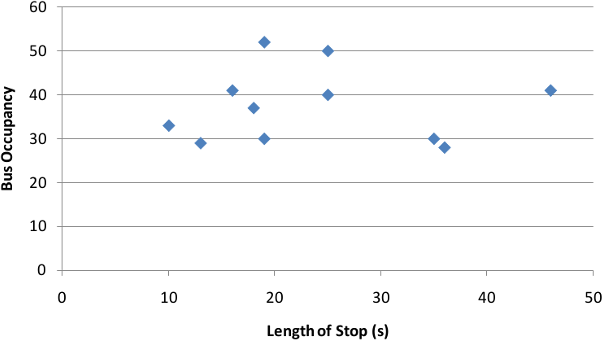
\includegraphics[width=0.5\textwidth]{occupancy}
  \caption{Bus Occupancy as a function of Stop Length} %TODO: Clarify whether this is for the following or preceeding stop. I don't actually remember.
  \label{fig:occ}
\end{figure}
\begin{figure}[!t]
  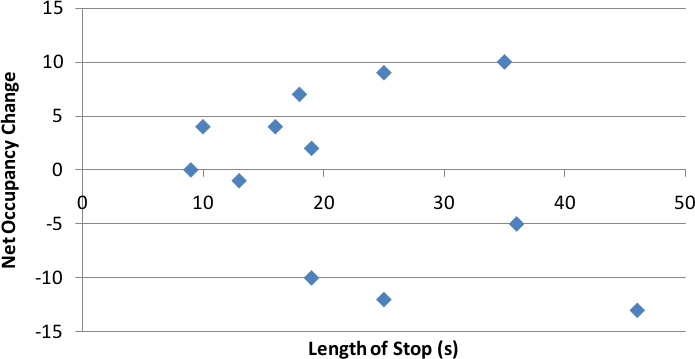
\includegraphics[width=0.5\textwidth]{netdelta}
  \caption{Net Delta Occupancy as a function of Stop Length}
  \label{fig:netdelta}
\end{figure}

Analyzing this data (fig.~\ref{fig:occ}), it quickly became apparant that stop length does not have any correlation to occupancy.
This makes sense, because the number of sedentary riders does not cause slowdowns; rather, the relevant metric is the number of people entering or exiting the bus.
Plotting the net occupancy change as a function of stop length (fig.~\ref{fig:netdelta}) was also inconclusive, as the longer stops could signify either positive or negative changes.
From stop timings alone, we would not be able to predict the direction of change.

\pagebreak
    
\begin{figure}[!t]
  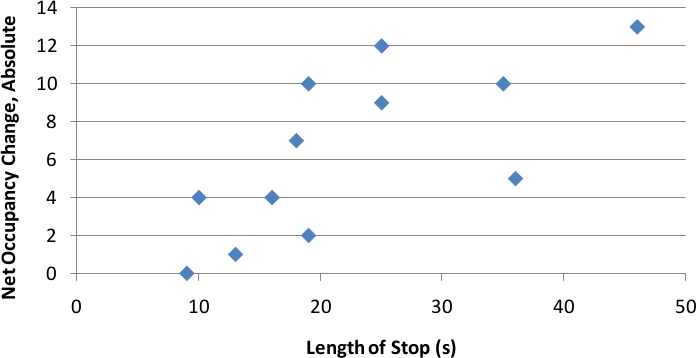
\includegraphics[width=0.5\textwidth]{absdelta}
  \caption{Absolute Delta Occupancy as a function of Stop Length}
  \label{fig:absdelta}
\end{figure}

\begin{figure}[!t]
  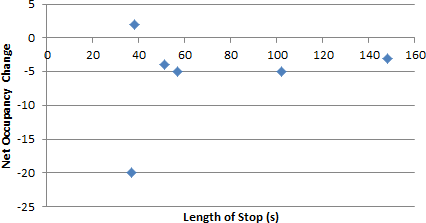
\includegraphics[width=0.5\textwidth]{onestopcrop}
  \caption{Net Delta Occupancy, Single Stop}
  \label{fig:onestop}
\end{figure}

Absolute change (fig.~\ref{fig:absdelta}), however, shows a much stronger correlation than either of the previous graphs.
Absolute change is not a useful metric on its own, but if it could be proven that certain bus stops tended to have a generally positive or negative net change, we could predict the sign of the change and thus the occupancy changes over time.
In other words, if more people tend to get on at a given stop than get off, a longer stop here means a large positive change to the number of passengers.
Conversely, a stop which is associated mostly with disembarking, a long stop would mean a large negative change.

To test this, we waited at a single bus stop and counted the number of passengers entering and leaving each bus on a certain route, and the length of the stops (fig.~\ref{fig:onestop}).
Data for this experiment was slower to collect, as the buses were spaced out.
This data suggests that this particular bus stop is predominantly a destination, rather than a starting point; longer stops here, then, would imply a net decrease in number of riders.
    
However, the data collected is insufficient to draw these conclusions; there can be significant variation depending on time and day of the week.
This data collection would need to be repeated at every bus stop, on a variety of days and times, in order to provide the required basis of prediction.
This clearly increases the time requirement to well beyond the scope of this study.
	
Thus, while the preliminary foray suggests that this approach is tentatively successful, it is not feasible for this study.
We move on to our next approach.

\subsection*{Promiscuous WiFi}
    
\subsubsection*{Packet Plot}
\begin{figure*}[!t]
  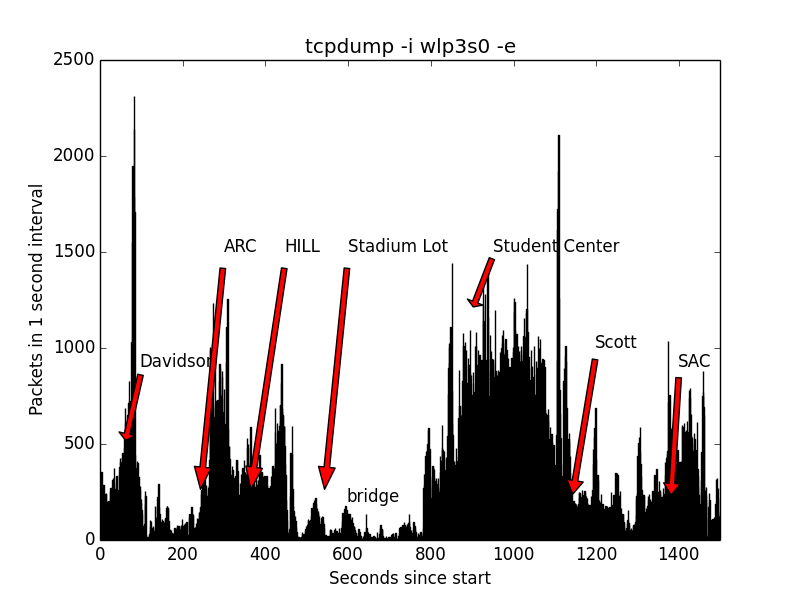
\includegraphics[width=\textwidth]{packets}
  \caption{Packets detected per 3-second bin}
  \label{fig:buspackets}
\end{figure*}

Plotting the number of packets in a histogram with three second bins (fig.~\ref{fig:buspackets}), we see that there are visible differences between stops.
This roughly lines up to the expected traffic around each stop -- stops like the BCC, Hill, the ARC, and the entirety of College Avenue have a large amount of traffic, while stops near the Visitor's Center and Werblin have very little.

\subsubsection*{Unique MAC Plot}

Network traffic is not a good indicator of occupancy, however, because it represents the amount of activity, rather than the number of actors; a single person transmitting a large amount of data may be interpreted as multiple people with the Packet Plot.
As such, our next step was to switch out ``number of packets'' for ``number of unique MAC addresses''.
The Router filter would be used here, since we don't want to count routers among the number of riders.

\begin{figure*}[!t]
  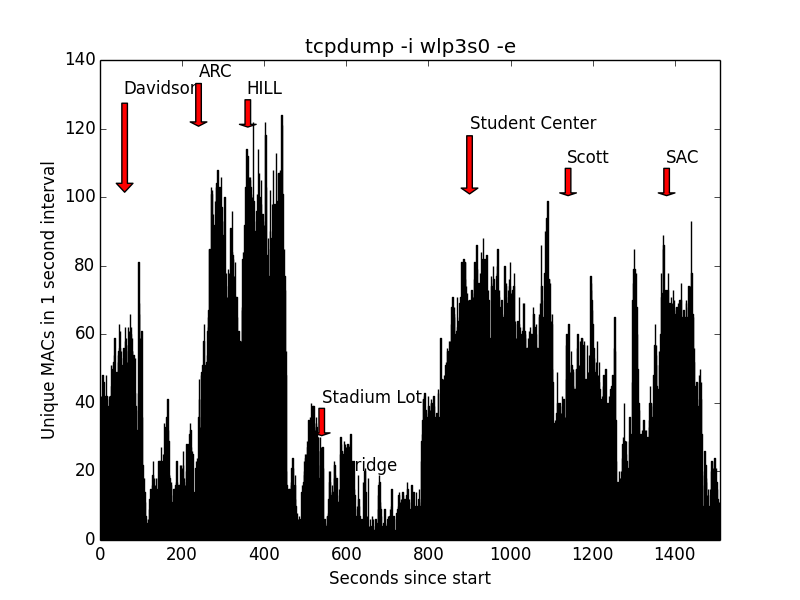
\includegraphics[width=\textwidth]{unique}
  \caption{Unique MAC addresses detected per 3-second bin}
  \label{fig:busunique}
\end{figure*}

The values on this plot differ noticeably between stops.
However, this is not due to occupancy; there are clearly not nearly that many people on the bus.
Instead, it seems that the shape of the plot is primarily influenced by the proximity to routers -- the portions of the bus loop by athletic fields and between campuses has nearly no data.

\subsubsection*{First-Last Grid Plot}
In order to establish which devices were on the bus, we plotted the time of the first and last occurrence of each device:

\begin{figure*}[!t]
  \includegraphics[width=\textwidth]{bus-grid-fixed}
\end{figure*}

Each point here represents a unique device, where the x-coordinate is the time of the first sighting, and the y-coordinate is the time of the last sighting.
Thus, the high concentration of data points along the line \(y=x\) represents the transient devices, most likely people the bus was passing by.
The clump of data points in the top left corner of the plot represents devices which were seen throughout the journey.
These are most likely our own devices, or stationary devices around the geographically identical first and last stops.

\subsubsection*{Presence Vector Plot}
In an attempt to minimize noise from the above transient devices and to compensate for the lack of traffic in uninhabited areas, we construct a plot similar to the previous. % This isn't a complete thought
For every address we encountered in the collection, we create a vector defined by the following function:
\begin{equation*}
  f(t) = \begin{cases}
    1 & t_{firstSeen} \le t \le t_{lastSeen}\\
    0 & otherwise
  \end{cases}
\end{equation*}

We sum these vectors into a single vector, where the value at any point indicates how many devices we can infer are presently on the bus.

\begin{figure*}[!t]
  \includegraphics[width=\textwidth]{bus-vectors-wide}
\end{figure*}

Overlaid on this plot is the step function corresponding to the observed number of riders.
It is scaled differently, as there is approximately a three time difference between the devices seen and the people riding.

We see that there appears to be an excellent correlation here, with the exception of the 400-700 second segment. % uhh... what about 0-400? That's also pretty bad.
This segment corresponds to the entrance to the College Avenue campus, a highly concentrated area which appears to have contributed considerable noise.
We do see, however, that the two changes in occupancy in this region seem to correspond to peaks in the traffic -- this means that the traffic is probably a flat-rate higher in that area, which we can account for in prediction.
		
Thus, we can conclude that this approach is successful. % I don't know about that, it seems really shaky to just declare that here.
